
%En ella se deben exponer brevemente pero con absoluta claridad, 
% la novedad y actualidad del tema,
% el objeto de la investigaci�n,
% sus objetivos,
% la hip�tesis de trabajo,
% el fundamento metodol�gico y
% los m�todos utilizados para realizar el trabajo de investigaci�n.
%Es decir, que la introducci�n es la fundamentaci�n cient�fica de la tesis en forma resumida.

\section{Introduction}
\begin{frame}

  The aim of this thesis is to support decision making regarding
  the location and redeployment of insurance agents to attend car wrecks.

  The idea is to develop models and methods for 
  (a) improving the service offered by insurance agents, 
  helping them arrive to the accident sites sooner, and 
  (b)  determining the number of adjusters required to perform 
  the service within the desired standards.

\end{frame}

\subsection{Problem}
\frame{
  \textit{The main goal is to determine the optimal bases (locations) 
    for placing the insurance company adjusters, 
    so as to minimize average or maximum response time
    from customer calls when accidents occur.}
}

\subsection{Motivation}
\begin{frame}
  When a car accident occurs, traffic congestions starts to pile up.
  This is because customers are not allowed to move their vehicles
  until the adjuster arrives.  
  The adjuster must record and determine the causes of the accident, 
  in order to move the car from the accident area and restore the flow.
  \begin{center}
    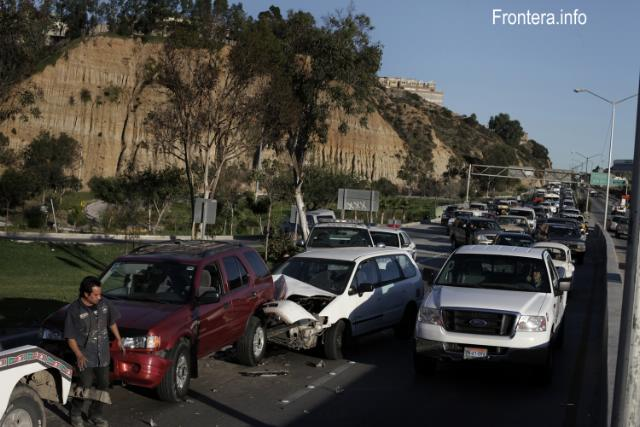
\includegraphics[scale=0.25]{389200-G}
  \end{center}
\end{frame}

\subsection{Background}
\begin{frame}[allowframebreaks]
  Richard Larson (1974) \cite{larson1974hypercube,jarvis1985approximating}
  proposes the Hypercube, and A-Hypercube models
  for a queuing approach for locating multiple facilities.

  James P. Jarvis (1985) \cite{jarvis1985approximating} incorporates
  location dependent service times characteristics for the A-Hypercube model,
  developing an approximation model for a spatially distributed queuing system
  under general service time assumptions.

  Berman et al. (1987) \cite{berman1987stochastic}
  formulate the stochastic queue p-median problem,
  and propose a heuristic approach for locating cooperative service facilities
  on a network.

  Goldberg et al. (1990) \cite{goldberg1990validating}
  propose a nonlinear integer programming model
  based on general service time approximation
  for spatially distributed queueing systems.

\end{frame}
